\documentclass{article}
\usepackage[utf8]{inputenc}
\usepackage[english]{babel}
\usepackage{amsmath}% http://ctan.org/pkg/amsmath
\usepackage{listings}
\usepackage{graphicx}
\usepackage{comment}
\usepackage{float}
\usepackage{biblatex}
\usepackage{lscape}
\usepackage{csquotes}
\usepackage{multirow}
\usepackage{ragged2e}
\usepackage{tabularx}
\usepackage[a4paper,pdftex,bottom=20mm, width=160mm]{geometry} 
\setlength{\parindent}{0pt} 
\setlength{\parskip}{1em}


\title{
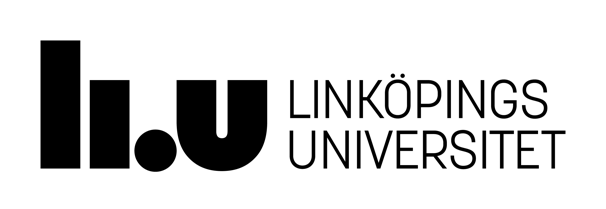
\includegraphics[scale=1.5]{liu_logga.png} \\
\vspace{2.0cm} \textbf{Testing Plan} \\
 \endgraf\rule{\textwidth}{.4pt}
  \large \textbf{TDDC88 Programutvecklingsmetodik}\\
   }
   
   
\author{Company 3}
\date{\today}

\begin{document}

\maketitle


\newpage
```latex
\section{Document Change History}

\begin{center}
\small\textit{Note: This change history table was generated by Autoleaf AI under the supervision of the Technical Writer. Only the most significant changes are highlighted, check the readme.md, found in gitlab, for more detailed information.}

\vspace{0.5cm}

\begin{tabular}{|p{0.05\textwidth}|p{0.09\textwidth}|p{0.17\textwidth}|p{0.14\textwidth}|p{0.39\textwidth}|}
\hline
\textbf{Ver.} & \textbf{Date} & \textbf{Modified Areas} & \textbf{Changed By} & \textbf{Description of Changes} \\
\hline
2.2 & 2024-10-17 & Req. Struct., User Classes, Func. Req., Non-Func. Req., Design Constraints & Analyst Team & Restructure document for clarity and traceability, introduce sub-requirements linked to main requirements, rename and restructure user roles section. Remove Software System Attributes section. \\
\hline
2.1 & 2024-10-10 & User Stories, Scope, Non-Func. Req., Overall Desc. & Analyst Team & Restructure user stories, clarify scope, streamline non-functional requirement descriptions, and improve overall description clarity. \\
\hline
2.0 & 2024-10-03 & Software Sys. Attr., User Stories, Constraints, Assumptions, Func. Req., Perf. Req. & Analyst Team & Introduce software system attributes, refine user stories, expand constraints, clarify assumptions, and provide specific details for functional and performance requirements. \\
\hline
1.1 & 2024-09-24 & Intro, Overall Desc., Specific Req. & Analyst Team & Expand initial structure with detailed descriptions of user roles, system functionalities, requirements, and constraints. \\
\hline
1.0 & 2024-09-19 & Intro, Overall Desc., Specific Req., Supporting Info & Analyst Team & Establish initial structure and content of the Requirements Specification document. \\
\hline
\end{tabular}
\end{center}

\vspace{1cm}
```
 

\newpage
\tableofcontents
\newpage

\section{Purpose}
This document outlines the architectural philosophy, key decisions, constraints, and significant elements of the camera management and security system. It serves as a comprehensive guide for understanding the motivations behind the architectural decisions and how different system components interact. This will help both current and future team members implement, maintain, and evolve the architecture.

\section{Architectural Goals and Philosophy}

The architecture follows a \textbf{modular, distributed} approach, where responsibilities are clearly separated between the \textbf{LAN Server} (for camera-related tasks) and the \textbf{External Server} (for management tasks). The system is designed to support \textbf{real-time processing}, \textbf{scalability}, and \textbf{secure user access}, while allowing each server to function independently for robustness and flexibility.

\subsection{Goals}

\begin{itemize}
    \item \textbf{Scalability and Performance}: Both the \textbf{LAN Server} and \textbf{External Server} should be able to scale independently to handle different loads, ensuring that camera control operations (scheduling, streaming) and alarm management do not interfere with each other.
    \item \textbf{Real-Time Responsiveness}: The system must process and display alarms within \textbf{5 seconds} (FRQ003-v1) and allow operators to respond quickly to critical events.
    \item \textbf{User Role-Based Access}: The system will manage different user roles with varying access levels (FRQ012-v1), including \textbf{Guards, Operators, Managers, and Admins}, with each role having distinct permissions across the \textbf{LAN Server} and \textbf{External Server}.
    \item \textbf{Security and Authentication}: All requests to the \textbf{LAN Server} and \textbf{External Server} must be authenticated using \textbf{JWT tokens} to ensure secure access such as camera control, alarm management, and user data.
\end{itemize}

\section{Assumptions and Dependencies}

\subsection{Assumptions}

\begin{itemize}
    \item \textbf{Camera and LAN Server Communication}: All cameras are assumed to be connected to the \textbf{LAN Server}, which manages direct interactions such as control actions (e.g., zoom, brightness), scheduling, and live streaming.
    \item \textbf{Front-End Interaction}: The \textbf{front-end} communicates with both the \textbf{LAN Server} and \textbf{External Server}, depending on the operation. The \textbf{LAN Server} handles camera controls, while the \textbf{External Server} manages alarms, user roles, and system management tasks.
    \item \textbf{Database}: A centralized database is shared between the \textbf{LAN Server} and \textbf{External Server}. It stores critical data such as \textbf{schedules, user roles, camera info, alarms, snapshots, and video clips}. The database should be accessible using familiar technologies like \textbf{SQLAlchemy} or \textbf{Flask-SQLAlchemy} for ease of development.
    \item \textbf{Team Experience}: The development team members have \textbf{limited experience} in programming, and their most familiar language and framework are \textbf{Python} and \textbf{Flask}. Therefore, the architecture is designed to use these technologies for the \textbf{LAN Server} and \textbf{External Server} to ensure that the team can effectively implement and maintain the system.
\end{itemize}

\subsection{Dependencies}

\begin{itemize}
    \item \textbf{Camera System}: The system relies on cameras to detect objects, trigger alarms, and send metadata and media (snapshots, video clips) to the appropriate servers. The cameras communicate with the \textbf{LAN Server} for media and scheduling tasks and the \textbf{External Server} for alarm metadata.
    \item \textbf{Real-Time Requirements}: The system must meet the requirement of alerting operators within \textbf{5 seconds} of an event being detected (FRQ003-v1). This puts significant importance on the \textbf{LAN Server}'s real-time processing capabilities.
    \item \textbf{User Role Management}: Proper role handling is essential, with distinct access levels for \textbf{Guards, Operators, Managers, and Admins}. This is managed through the \textbf{External Server}, which ensures that each role has appropriate permissions across the system.
    \item \textbf{Python/Flask Framework}: Both servers (LAN and External) are built using \textbf{Python} and \textbf{Flask} to align with the team’s experience, ensuring that the team can implement features efficiently while leveraging their familiarity with these technologies.
\end{itemize}

\section{Architecturally Significant Requirements}

These are the key functional and non-functional requirements that shape the architecture:

\begin{enumerate}
    \item \textbf{Camera Operations} (Handled by \textbf{LAN Server}, \textbf{Camera}, and \textbf{External Server})
    \begin{itemize}
        \item The camera system must \textbf{recognize objects in motion} and determine what they are with a confidence percentage (FRQ001-v1).
        \item When an alarm is triggered, the \textbf{Camera} will capture the best snapshot and video clips, sending metadata to the \textbf{External Server} (FRQ002-v1, N02-1).
        \item \textbf{Camera schedules} must be updated and executed within 10 minutes, with a 95\% success rate through requests from \textbf{LAN Server} (FRQ006-v1).
        \item The \textbf{Admin} will be able to update the camera’s \textbf{confidence settings} by sending requests to \textbf{LAN Server} (FRQ007-v1).
    \end{itemize}
    \item \textbf{Alarm Management} (Handled by \textbf{External Server})
    \begin{itemize}
        \item The \textbf{operator} must be alerted to an intrusion within 5 seconds of detection (FRQ003-v1).
        \item The system must display \textbf{alarm notifications} to operators with options to \textbf{confirm or deny the alarm} (FRQ005-v1).
        \item Alarm metadata must be stored in the database, including time, date, camera ID, and approval status (N02-1, N02-2).
    \end{itemize}
    \item \textbf{User Role and Access Management} (Handled by \textbf{External Server})
    \begin{itemize}
        \item The system must support \textbf{four distinct user roles}: \textbf{Guard, Operator, Manager, Admin} (FRQ012-v1).
        \item Each role must have different access levels (e.g., \textbf{Operators} can handle alarms, \textbf{Managers} can view statistics, \textbf{Admins} have full access) (FRQ012-v1, 12-1 to 12-4).
        \item \textbf{Admin} will manage user roles and permissions (FRQ015-v1).
    \end{itemize}
    \item \textbf{Operator and Manager Functionality} (Handled by \textbf{External Server} and \textbf{LAN Server})
    \begin{itemize}
        \item The \textbf{operator} must be able to view live camera feeds by sending requests to \textbf{LAN Server} (FRQ008-v1, FRQ009-v1).
        \item The \textbf{manager} must have access to \textbf{statistics and alarm history} by sending requests to \textbf{External Server} (FRQ010-v1, FRQ014-v1).
    \end{itemize}
\end{enumerate}

\section{Decisions, Constraints, and Justifications}

\begin{itemize}
    \item \textbf{Decision}: Use \textbf{Python/Flask} for both the LAN Server and External Server.
    \begin{itemize}
        \item \textbf{Constraint}: The system must be built using \textbf{Flask} as the web framework. Developers should avoid using other frameworks (e.g., Django) to maintain consistency across both servers.
        \item \textbf{Justification}: The development team is most familiar with \textbf{Python} and \textbf{Flask}, so this choice reduces the learning curve and ensures faster development. It also aligns with the team’s current skill set, which is important given the team's lack of extensive programming experience.
    \end{itemize}
    \item \textbf{Decision}: Separate the \textbf{LAN Server} and \textbf{External Server} to handle different responsibilities.
    \begin{itemize}
        \item \textbf{Constraint}: The \textbf{LAN Server} should only manage camera-related tasks (e.g., streaming, control actions, scheduling), while the \textbf{External Server} handles alarm management, user roles, and system management.
        \item \textbf{Justification}: This separation allows each server to scale independently and ensures that critical real-time camera tasks are not slowed down by alarm processing or user management. This also aligns with the system's need to handle real-time alerts within \textbf{5 seconds}. And by doing this, the \textbf{LAN Server} can act as an entry point to the camera's LAN network environment.
    \end{itemize}
    \item \textbf{Decision}: Use \textbf{PostgreSQL} for the database.
    \begin{itemize}
        \item \textbf{Constraint}: The system’s data, including camera schedules, user roles, alarms, snapshots, and video clips, must be stored in a \textbf{PostgreSQL} database. Developers must implement all database interactions using \textbf{Flask-SQLAlchemy} to ensure consistent usage of the database.
        \item \textbf{Justification}: \textbf{PostgreSQL} is chosen for its reliability, scalability, and ability to handle complex queries. It's well-supported with \textbf{Python/Flask} through \textbf{Flask\_SQLAlchemy}, which simplifies database interaction and aligns with the team’s existing skill set.
    \end{itemize}
    \item \textbf{Decision}: Use \textbf{C} for developing the camera application.
    \begin{itemize}
        \item \textbf{Constraint}: The camera-side application must be developed using \textbf{C}, as the camera SDK only supports this language. Developers must avoid introducing other languages for the camera-side application to maintain compatibility.
        \item \textbf{Justification}: The camera SDK is provided in \textbf{C}, making it essential to use C for developing the application. This decision ensures that the camera applications can interact directly with the camera’s hardware for tasks like motion detection, object recognition, and alarm triggering.
    \end{itemize}
    \item \textbf{Decision}: Use \textbf{React} as the frontend framework.
    \begin{itemize}
        \item \textbf{Constraint}: The frontend must be built using \textbf{React} to manage the user interface. Developers should avoid using other frontend frameworks to maintain consistency.
        \item \textbf{Justification}: \textbf{React} is well-suited for applications with multiple pages and user roles, like ours, which will have distinct views for \textbf{Guards, Operators, Managers, and Admins}. With \textbf{React}, we can efficiently manage access control through its third-party libraries, such as \textbf{React Router} for navigation and role-based routing, and libraries like \textbf{Redux} or \textbf{React Context} for state management. Additionally, the \textbf{component-based architecture} React uses also promotes reusability and easier maintenance.
    \end{itemize}
    \item \textbf{Decision}: Use \textbf{JWT tokens} for stateless authentication.
    \begin{itemize}
        \item \textbf{Constraint}: Developers must implement \textbf{stateless authentication} using \textbf{JWT tokens}. They should avoid storing session data on the server. Token validation should be implemented consistently across both the LAN and External Servers.
        \item \textbf{Justification}: JWT tokens allow for \textbf{stateless, scalable} authentication. This reduces complexity and improves performance by eliminating the need for server-side session storage, making it easier to scale horizontally across multiple servers.
    \end{itemize}
    \item \textbf{Decision}: Use \textbf{RESTful APIs} instead of SOAP.
    \begin{itemize}
        \item \textbf{Constraint}: All communication between the frontend, \textbf{LAN Server}, and \textbf{External Server} must use \textbf{RESTful APIs}. SOAP-based APIs are not allowed to maintain simplicity and scalability.
        \item \textbf{Justification}: \textbf{RESTful APIs} are lightweight, easier to implement, and more scalable compared to SOAP. They align with the team’s familiarity with \textbf{Python/Flask} and are better suited for real-time communication between the frontend and backend servers.
    \end{itemize}
\end{itemize}
\section{Architectural Mechanisms}

\subsection{Flask Framework for LAN and External Servers}
\begin{itemize}
    \item \textbf{Purpose}: Flask serves as the web framework for both the \textbf{LAN Server} and \textbf{External Server} to handle routing, request processing, and integration with other components like databases and authentication.
    \item \textbf{Attributes}:
    \begin{itemize}
        \item \textbf{Modular Design}: The project is organized modularly, separating functionalities into different blueprints (e.g., \textbf{alarms, cameras, schedules}), making the codebase easier to manage and scale.
        \item \textbf{Extensibility}: Using separate controllers, services, and routes for each module (e.g., \texttt{alarms}, \texttt{auth}, \texttt{cameras}), new features can be added or modified without affecting other parts of the system.
    \end{itemize}
    \item \textbf{Function}:
    \begin{itemize}
        \item \textbf{Controllers}: Each controller, such as \texttt{alarms\_controller.py}, manages business logic for specific domains (e.g., managing alarms).
        \item \textbf{Services}: Services like \texttt{alarms\_service.py} and \texttt{auth\_service.py} interact with the database and execute business logic.
        \item \textbf{Routes}: Defined in files like \texttt{alarms\_routes.py}, routes link HTTP requests to appropriate controller functions.
        \item \textbf{Execution}: The \texttt{run.py} file initiates the Flask app, loading configurations from \texttt{config.py} and initializing extensions (e.g., database connections) from \texttt{extensions.py}.
    \end{itemize}
\end{itemize}

\subsection{Separation of LAN Server and External Server Responsibilities}
\begin{itemize}
    \item \textbf{Purpose}: The \textbf{LAN Server} and \textbf{External Server} have distinct roles—managing camera-related tasks and broader system functions, respectively.
    \item \textbf{Attributes}:
    \begin{itemize}
        \item \textbf{Inherent Role Separation}: The \textbf{LAN Server} handles camera network operations, while the \textbf{External Server} manages user roles, alarm processing, and authentication.
        \item \textbf{Network Security}: The \textbf{LAN Server} secures the camera network, exposing devices only through specific endpoints.
        \item \textbf{Scalability}: Each server scales based on its load—\textbf{LAN Server} for camera tasks and \textbf{External Server} for user and alarm management.
    \end{itemize}
    \item \textbf{Function}:
    \begin{itemize}
        \item \textbf{LAN Server}: Handles video streaming, camera control, and scheduling.
        \item \textbf{External Server}: Manages alarm and user data updates in the database.
    \end{itemize}
\end{itemize}

\subsection{PostgreSQL Database with Flask\_SQLAlchemy}
\begin{itemize}
    \item \textbf{Purpose}: PostgreSQL is used for persistent storage of camera schedules, users, alarms, snapshots, and video clips, accessed via the Flask\_SQLAlchemy ORM.
    \item \textbf{Attributes}:
    \begin{itemize}
        \item \textbf{ORM Abstraction}: Database models are defined in \texttt{models.py}, mapping classes to tables.
        \item \textbf{Centralized Configuration}: Database configurations are stored in environment variables and processed through \texttt{config.py}.
    \end{itemize}
    \item \textbf{Function}:
    \begin{itemize}
        \item \textbf{Models}: Entities like users and alarms are represented in \texttt{models.py}.
        \item \textbf{Service Layer}: Service files interact with models to perform database operations.
        \item \textbf{Controllers and Routes}: Handle HTTP requests and return results based on database interactions.
    \end{itemize}
\end{itemize}

\subsection{Camera Application in C}
\begin{itemize}
    \item \textbf{Purpose}: The camera application is developed in \textbf{C} to leverage the camera’s SDK, which only supports C, to retrieve motion detection and object recognition data.
    \item \textbf{Attributes}:
    \begin{itemize}
        \item \textbf{Built-in Integration}: Interacts with camera endpoints to gather detection data.
        \item \textbf{Lightweight JSON Construction}: Packages data into JSON format for efficient transfer.
        \item \textbf{Event Triggering}: Constructs and sends JSON payloads to the \textbf{External Server} to trigger alarms.
    \end{itemize}
    \item \textbf{Function}: Sends an HTTP request with a JSON object upon event detection.
\end{itemize}

\subsection{React for Frontend}
\begin{itemize}
    \item \textbf{Purpose}: The \textbf{React} framework is used for building a dynamic, multi-role frontend.
    \item \textbf{Attributes}:
    \begin{itemize}
        \item \textbf{Component-Based Architecture}: Promotes reusability and modularity.
        \item \textbf{State Management}: \textbf{Redux} or \textbf{React Context} handles state across pages and roles.
        \item \textbf{Access Control}: Uses libraries like \textbf{React Router} for role-based navigation.
    \end{itemize}
    \item \textbf{Function}: Renders views based on user roles and interacts with Flask APIs.
\end{itemize}

\subsection{JWT for Stateless Authentication}
\begin{itemize}
    \item \textbf{Purpose}: \textbf{JWT tokens} manage stateless authentication across servers.
    \item \textbf{Attributes}:
    \begin{itemize}
        \item \textbf{Stateless}: Eliminates server-side session storage.
        \item \textbf{Role-Based}: Tokens include roles for API access control.
        \item \textbf{Expiration}: Tokens have expiration times for enhanced security.
    \end{itemize}
    \item \textbf{Function}: Validates tokens for each request, including role-based access.
\end{itemize}

\subsection{RESTful API Communication}
\begin{itemize}
    \item \textbf{Purpose}: RESTful APIs are used for lightweight, scalable communication.
    \item \textbf{Attributes}:
    \begin{itemize}
        \item \textbf{Stateless}: Each API call is independent, allowing easier scaling.
        \item \textbf{Standardized}: Uses HTTP methods (GET, POST, etc.).
        \item \textbf{JSON-Based}: JSON format is easy for \textbf{React} to process.
    \end{itemize}
    \item \textbf{Function}: Handles frontend and backend communication through distinct endpoints.
\end{itemize}

\section{Key Abstractions}
\begin{itemize}
    \item \textbf{User}: Represents system operators, managers, or administrators.
    \item \textbf{Camera}: The device for detecting motion and streaming video.
    \item \textbf{Alarm}: Event triggered by detection, containing metadata and media.
    \item \textbf{Schedule}: Defines active/inactive times for cameras.
    \item \textbf{CameraControlAction}: Actions initiated by users to control settings.
\end{itemize}

\section{Architectural Layers}
\begin{itemize}
    \item \textbf{Presentation Layer (Frontend)}: React frontend interacts with both servers based on request type (camera vs. user management).
    \item \textbf{Service Layer}:
    \begin{itemize}
        \item \textbf{LAN Server}: Manages camera operations, streaming, and scheduling.
        \item \textbf{External Server}: Manages alarms, user roles, and system configurations.
    \end{itemize}
    \item \textbf{Data Layer (Database)}: Stores camera and user data, alarms, schedules, and media.
\end{itemize}

\section{Architectural Views}
\subsection{Logical View}
\begin{itemize}
    \item \textbf{LAN Server}: Manages device communication, streaming, and scheduling.
    \item \textbf{External Server}: Handles user and alarm management.
\end{itemize}

\subsection{Operational View}
\begin{itemize}
    \item \textbf{LAN Server}: Operates within the local network (LAN).
    \item \textbf{External Server}: Handles authentication and alarm metadata.
\end{itemize}

\subsection{Use Case View}
\begin{itemize}
    \item \textbf{Use Case 1}: Scheduling camera activation via frontend request to the \textbf{LAN Server}.
    \item \textbf{Use Case 2}: An alarm triggers, sending metadata to the \textbf{External Server}, which stores it.
\end{itemize}
\end{document}
